\documentclass[12pt,notitlepage]{article}
\usepackage{fullpage}
\usepackage{amssymb}
\usepackage{titling}
\usepackage{graphicx}
\usepackage{xcolor}
\usepackage{mathtools}
\newcommand{\bmc}{\begin{center} \begin{math}}
\newcommand{\emc}{\end{math} \end{center}}
\newcommand{\mfloor}[1]{\lfloor #1 \rfloor}

\title{FiL$\varnothing$: Dynamic Topologies for Federated Learning}
\author{spiros thanasoulas (st19@illinois.edu)}
\begin{document}
\maketitle
\begin{abstract}
As the amount of data and participating nodes increases, decentralized and 
asynchronous versions of machine learning algorithms are becoming more 
prominent. Overlay networks that exploit efficient topologies have been 
shown recently to dramatically speed up training convergence and to reduce 
errors.  Up to now though, they have to be designed a-priory and utilize 
structural knowledge of the underlying network. We propose a dynamic scheme 
where the participating workers self organize via p2p network with the goal
of forming groups of similar optimization step times. To achieve this we utilize
native features of distributed hash tables.
\end{abstract}
\section{Introduction}
In the domain of federated learning (FL) where data should not escape the
premises of the device or the silo, efficient communication between the workers
is paramount. In general the types of algorithms 
\cite{towardsFL}, 
\cite{DecentralizedFederatedMultitaskLearning} that operate on the local data 
also require sharing the results of each step with all or just their 
neighboring nodes. A characteristic example would be the family of gradient 
descent algorithms like stochastic gradient descent (SGD) or the distributed
variant (dSGD). Thus the topology of the network, in the sense of which
neighbors are available to each worker, can drastically affect the
efficiency of the computation. Recent works attempting to exploit the topology
of the network \cite{marfoq2020throughputoptimal}, \cite{matcha} 
have been very successful in achieving even order of magnitude faster 
convergence of dSGD runs. They rely on knowledge of the underlying network to
create efficient overlay topologies. This works well for the cross-silo 
FL case because the network is mostly static. But it also 
requires a-priori knowledge of it, and once the overlay is created, it is not
easy to change.

We will attempt to resolve this limitation by leveraging tools from the field
of peer to peer (p2p) research  and more specifically, distributed hash tables 
(DHTs), thus creating a dynamic network structure that will still be throughput
efficient. This approach would also not require any prior knowledge of the 
underlying network, while at the same time achieving progressively better 
connectivity. Finally our approach will have fault tolerance built-in since
the system we will build on is designed to accommodate node failures.

One important observation that we make is that for every step of the algorithm
the node requires some time to perform its local update $T_{l}$ and 
some time to communicate with its neighbors $T_{n}$. This means that nodes
are in lockstep, as is the case for many parallel discrete event based 
algorithms.  Thus by using $T_{l}$ as an input for a locality metric on the DHT
 keys, the formed neighborhoods impact how efficiently the algorithm
converges. The key insight to our approach is that by {\it using the DHT as
our neighbor discovery and routing platform, we will form groups of similar 
$\Delta T$ that will be connected in parallel as shown in Figure 1.}
This should allow for optimal global convergence time of the algorithm.
In addition, proximity neighbor selection (PNS) 
can be employed as well to minimize for the underlying network latency 
that exists within $T_{n}$. 

\begin{figure}
\centering
\begin{minipage}{.5\linewidth}
\centering
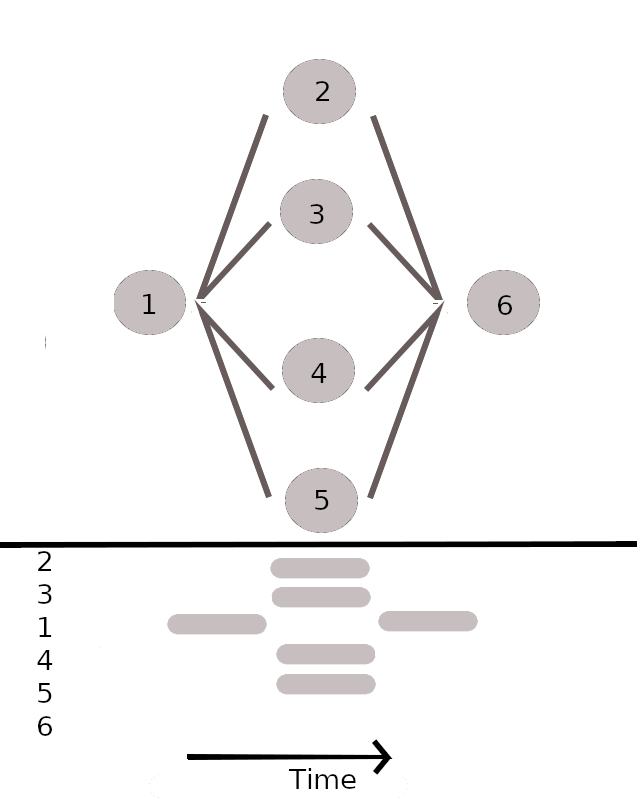
\includegraphics[scale=0.3]{img/fig1a.png}
\end{minipage}%
\begin{minipage}{.5\linewidth}
\centering
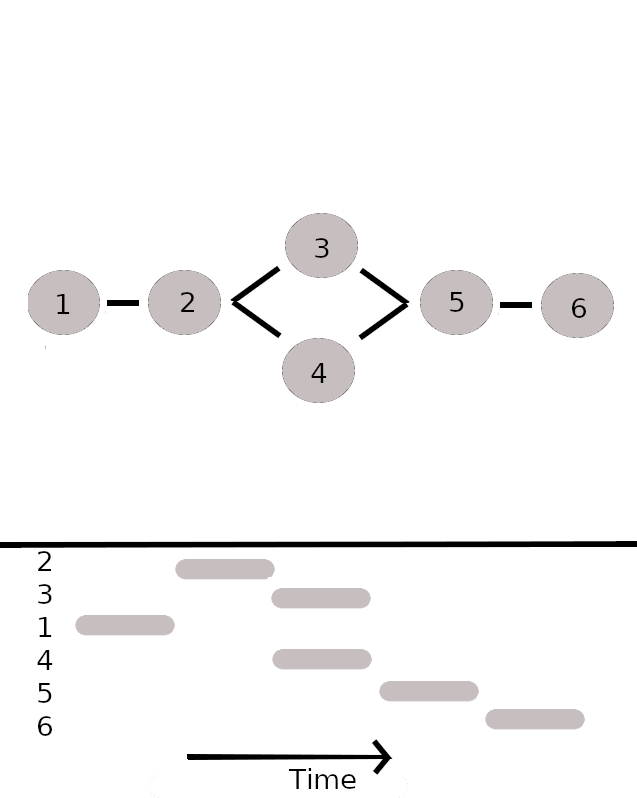
\includegraphics[scale=0.3]{img/fig1b.png}
\end{minipage}
\caption{two different configurations that demonstrate how parallelism achieves
better convergence time} 
\end{figure}

The paper is structured as follows
\begin{itemize}
\item In {\it Related Work} we note important contributions in selecting 
topologies for FL tasks as well other uses of p2p concepts on them.
We also list research on topologies and certain p2p networks that have 
promising properties if adopted for our needs.

\item In {\it Design} we define the communication model and which properties
our solution hopes to satisfy. By reasoning about the nature of the dSGD 
algorithm we notice how topology can drastically affect convergence times.
We draw analogs from similar problems in related fields to propose 
modifications on DHTs that would make them efficient overlays for FL tasks. 
Finally we will investigate a setup where a part of the computation for
each round is expected not to finish, either by stragglers or nodes that
failed. We will design around such a setup and observe that it doesn't 
only dramatically increase convergence times for the FL task operating on 
most of the data, but also acts as a fault tolerance mechanism.

\item In {\it Implementation} we present the design of our discrete event
simulator that helps evaluate the hypotheses that have been made. Initial
runs are performed that show the impact of local update time as a neighborhood
metric.

\item In {\it Evaluation} we will demonstrate the impact our dynamic topologies
have on the convergence time of the simulated FL task completion times. We 
will also  attempt to address some obvious shortcomings of the naive initial 
design proposed.
\end{itemize}
And the main contributions of the paper are
\begin{itemize}
\item a way to instruct similarly paced workers to form an overlay network using a DHT
\item a way of exploiting fast local convergence to achieve faster global convergence by discarding
      only a small part of the total computation, in a controlled fashion
\item a reliable inter-node communication scheme that by using the above position provides resilience
      for the whole network.
\end{itemize}

\section{Related Work}
As it has been observed in the seminal survey work \cite{fl-survey} some of 
the core assumptions in Federated Learning, like the cross-silo,or cross-device
setups could be challenged by utilizing p2p networks. It is also notes that
topology is a crucial factor. The first approach to exploit the topology was
MATCHA \cite{matcha} was based on matching decomposition sampling, that reduced
the communication delay per iteration of the dSGD algorithm. A throughput 
optimal topology design was also suggested \cite{marfoq2020throughputoptimal}
and where the input is the connectivity graph of the participating nodes.
From there an overlay is designed which maximizes the network throughput of
the system and thus reduces the time it take for runs of the dSGD algorithm
to converge. The metric that is taken is called the mean cycle time
and depends on the total delay between to consecutive steps of the algorithm
called the {\tt mean cycle time} (MCT). Their delay model incorporates
both $T_n, T_l$ of each step. Before that other p2p decentralized SGD 
approaches have been noted \cite{personal-private} but not really considering
the topology as an optimizing factor.

Another important body of work that we investigated was the structure of
topologies generated by p2p networks and how they fit in providing sufficient
overlays for FL tasks. Hypercube-like routing schemes like Pastry \cite{pastry}
 or ring-based like Chord \cite{chord} can, with proper modifications, offer
efficient DHTs to build our dynamic topologies on top. Skip-graphs 
\cite{skip-graphs} also seem to satisfy many of our requirements.
Finally we note that fat tree topologies \cite{fat-trees} are investigated 
for their provably efficient communication properties and their successful 
deployment in many HPC setups. On the subject of fault tolerance we investigated
how to connect traditional p2p fault tolerant routing as well as networking
fault-tolerance schemes \cite{fat-trees-fault}.

\section{Design}
\subsection{Problem Setup}
Distributed stochastic or mini-batch gradient descent algorithms like 
cooperative SGD \cite{coop-sgd} work in lockstep between performing local 
model updates, and communicating with their neighbors. In the case of 
cooperative SGD there can be $\kappa$ steps of local updates between successive
neighbor communications, here for generality we can consider that a neighbor
update will happen at every iteration. Thus at an arbitrary iteration $s$ of
the algorithm at a node $i$ must first receive possible updates from the 
neighborhood, then operate on its mini-batch and finally upload the results
back to the neighborhood. If we ignore the upload time for the neigbors next 
step since it is also encoded as a download time from the previous step we can
express the total delay as.
\bmc
\Delta T^s_{(i,j)} = \max_j(T_{j}^{s-1}) + T^s_i 
\emc

In the above setup all possible network induced delays are encoded in the 
neighborhood term. For now this keeps the model simple and we focus on the 
local delay of each node $T^s_i$. It is evident that different choices of
neighborhoods can affect the whole network convergence time.                                                                                                                                                                  

As seen above in Figure 1 if the {\it parallel group} shares approximately the
same $\Delta t$ it should finish its computation step at approximately the 
same time. But if part of it is a slower node, then its $\Delta T$ will be
shared by the whole group. Thus an important aspect of our system  will be
first the discovery of similarly paced nodes around us and the formation of
{\tt parallel groups} with them. 
The model that we will operating considers the local computation time to be
significantly more than internode messaging over the network. Another important
point here is that the size of messages exchanged will be small. Only the
results of the SGD computation (the calculated local gradients) are communicated,
the actual data remain local to the node that processes them, an important feature
of Federated Learning systems.

\subsection{DHTs as topology managers}
We are seeking a completely decentralized solution that can start from any 
initial topology and quickly converge to a throughput optimal one, without
any a-priori knowledge of the network. By employing locality-preserving hashing
with $\Delta T$ as the key, we will gain naturally from the DHT the ability to
create neighborhoods of similarly paced nodes. Due to the way we are planning
to use it a DHT that supports at least basically range queries is needed.
For this purpose we considered three possible candidates. 
\begin{itemize}
\item Pastry can be used since each node maintains neighbor lists. A node 
interested in getting a list of participants within a $\Delta T$ of its
neighborhood look in its neighbor list to see if that range is completely 
covered by the existing participants, or otherwise push out a message with
associated with TTL to both directions that would accumulate the nodes in that
range. Once the TTL expires or the range is exceeded the last owner of the
accumulation reports it back to the node. 

\item Chord with added predecessor/successor lists to each
node, or some variant of the algorithm like BNN-Chord can be used 
\cite{bnn-chord}.

\item Skip-graphs \cite{skip-graphs} which were designed to address this 
specific problem can also be employed. Another property they have is that
they can tolerate removal of large groups of nodes (up to a fraction of 
$O(\frac{1}{log N})$ without becoming highly disconnected. They could be
desirable as the need for removal and reinsertion of nodes with their
updated metrics as the topology improves, translates to high churn.
\end{itemize}

Considering the above options, we decided to move forward using Pastry
as a DHT. The reason for that is that pastry, logically separates
the Neighborhood set, the Routing table and the Leaf set. In traditional
pastry, the Leaf set and the Routing table are keyed on the actual DHT key.
But the Neighborhood set can also take other parameters into account (like RTT,
or some other form of network proximity). This flexible design seems like a good choice
for our DHT since by keying only on time to complete an SGD round, we can create neighborhoods
that are non preferable in other metrics. 

We believe that the frequent rekeying argument that would benefit the choice of skip-graphs,
can be controlled by updating of the key only once $i$ local SGD steps have been
performed. Proven pace-steering techniques that are used in other FL setups \cited{TowardsFL}
to address this exact problem can be used here to ensure that our DHT will never experience a large
number of nodes attempting to remove and reinsert themselves.

\subsection{Inter-Neighborhood Connectivity}
We have seen that in the presence of diversely paced nodes we want to form 
neighborhoods based on that pace. The question arises of how should we 
interconnect these between them. In every such neighborhood there will be
a minimum (the fastest) and a maximum valued node on $\Delta T$ (the slowest).
For arguments we saw above, that whole group can only be as fast as its
slowest node. Therefore the connection to the directly slower group above it
should only happen from that node. Equivalently the connection to a faster 
group below, should happen from the fastest node. This is a well known
interconnectivity scheme named Fat-Tree \cite{fat-trees} that is used in 
high throughput packet switching.
\begin{figure}[h]
\begin{center}
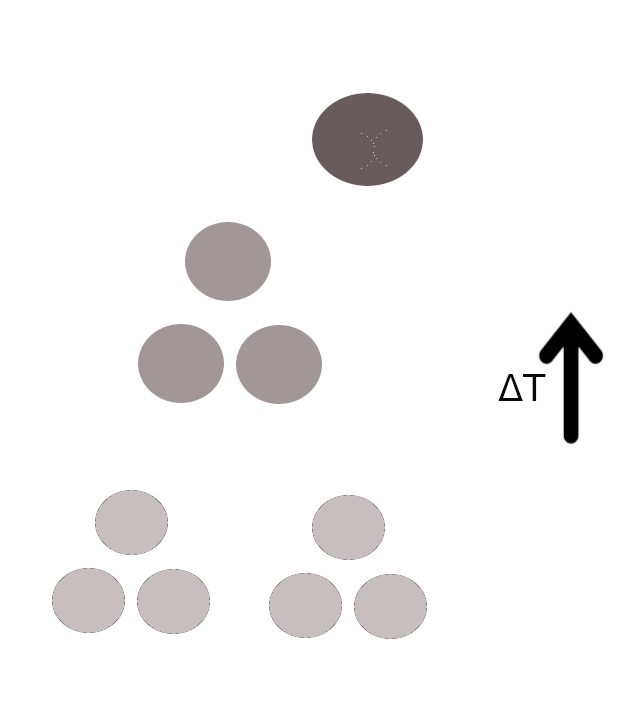
\includegraphics[scale=0.17]{img/fig2.png}
\end{center}
\caption{Fat tree topology on increasing $\Delta T$.}
\end{figure}

It is possible to manipulate the locality function of the DHT to enforce a
level like structure. By changing the hashing function  from the identity on
 $\Delta T$ to something of the form
\begin{center}
\begin{math}
H(\Delta T) := \mfloor{log(f(\Delta T, global properties))}
\end{math}
\end{center}
Work still remains in constructing exact form of the function, taking into account the
desired nodes per level, as well as levels in the whole range.
That would enforce the desired tree like structure on the ring.

\subsection{Most stragglers left behind scheme}
In the way we have presented the computation till now, it should be evident that
we can not get significant gains on the final convergence time. Since some delaying
nodes will still be connected, then their neighbors will have to wait for them, before starting
the next round. During that time the rest of the network can not move to next iteration.
This is why we propose to only require a percentage of the total nodes to complete the computation.
The nodes that are ready will be signalling their upstream (up in the sense of delay) neighbors eagerly
and once a number of nodes relative to the size of the group has completed their iteration cancellation signals
will be sent to the stragglers and a new round will begin. This approach has the benefit of unifying stragglers
with potentially failed nodes and utilizing a common strategy.
\susubsection{Failure Handling}
An established way to increase resiliency is to provide more possible links between nodes as mentioned also in \cite{fat-trees-fault}.
In that sense, more than one overlay networks can coexist, to account for possible link failures. In the case of a node failure,
there is not much that our system can do, but since we don't require all the nodes to finish the computation, data points from other SGD
participants will attempt to cover for that loss. For this reason, we chose Pastry as our initial DHT attempt. By being able to maintain
at the same time neighbors in two different metrics, we can chose to forward a message from a potentially failed link from the other set.
By the design of our network most a message generally will leave a node travelling towards a node that is still processing its local data.
We want 
\begin{itemize}
\item our message to reach more than one neighbors in case one of them crashes.
\item our computation to not be double counted.
\end{itemize}
To achieve this we will create a similar technique to a server-shim as it is mentioned in \cite{aegean} or dynamic routing as mentioned in
\cite{fat-trees-fault}.
For a message to leave a node, it has to get the receipt acknowledgement of more than one "upstream" nodes. Only then the message will be 
consider delivered for that node.
As for the double counting, the message which is being propagated has to be able to evaluate to a prefix sum at each node. When a message
is received in node (B) from node (A) it is opened up and decision for each prefix it taken. 
if a prefix coming from (A)s message has been seen already, {\it and} the (A) message containing the seen prefixes at node (B) successfully transmitted
to more than one upstreams, then this prefix is discarded. If the prefix in (A)s message has not been seen and (B)s message hasn't been transmitted, we add
it to our outgoing prefix sum for our upcoming send action. If we have sent a message yet we receive from (A) a prefix we have not in our records
we propagate it (always using our replicating server-shim like scheme). 
At any given moment if a node manages to gather a satisfactory number of collected prefixes, a message to all the participants who we haven't contacted yet
(a very small amount of the network) is sent out to signal them that they can stop their computation and move to the next round.

\subsection{On incorporating network related delays}
For simplicity we have kept our model intentionally vague. It seems there is
only one form of delay that dictates the pacing of the nodes and we have
presented it to be the $\Delta T$ of the local step. But in the 
original model we also have the network delays between the neighbors. The 
observation to be made here is that we really care for the largest of the two
delays whichever that is. The other one can be incorporated as an appropriately
scaled proximity network selection term. That means in our resulting routing
key on the DHT can have its high order bits set by the driving delay on each
node and use lower order bits for the remaining one. 

\section{Implementation}
We have designed a completely event based simulator that generates various graphs, 
can apply delay distributions on the nodes and then perform the required amount
of iterations on them. The code is already functional, yet a lot of work remains
to incorporate the proper topology constructors. The simulator is written an golang
and can work with event deltas up to the millisecond range, and with thousands of
concurrently running nodes, easily in commodity hardware. To date we have
\begin{itemize}
	\item a way to generate and interconnect overlay connectivity graphs, using linear,
		parallel,random and tree-like structures.
	\item a way to annotate them with workload characteristics (for example expected
		local gradient step time, and delta)
	\item the ability to perform a simulation run for arbitrary iterations on that
		network and collect statistic.
\end{itemize}
Our simulator can export data to JSON and the dot graph language, as well as import from these forms for ease
of automation. Digraphs are supported natively and actually although not seen in this report, 
the engine treats graphs as directed.

\section{Evaluation}
Since this is highly work in progress we will just demonstrate some very preliminary results of 
the simulator and the effect of interconnectivity on the convergence. In the below example 
the overlay graphs are kept small for visualization purposes but we can easily run experiments on tens
of thousands of nodes.
\begin{figure}
\centering
\begin{minipage}{.5\linewidth}
\centering
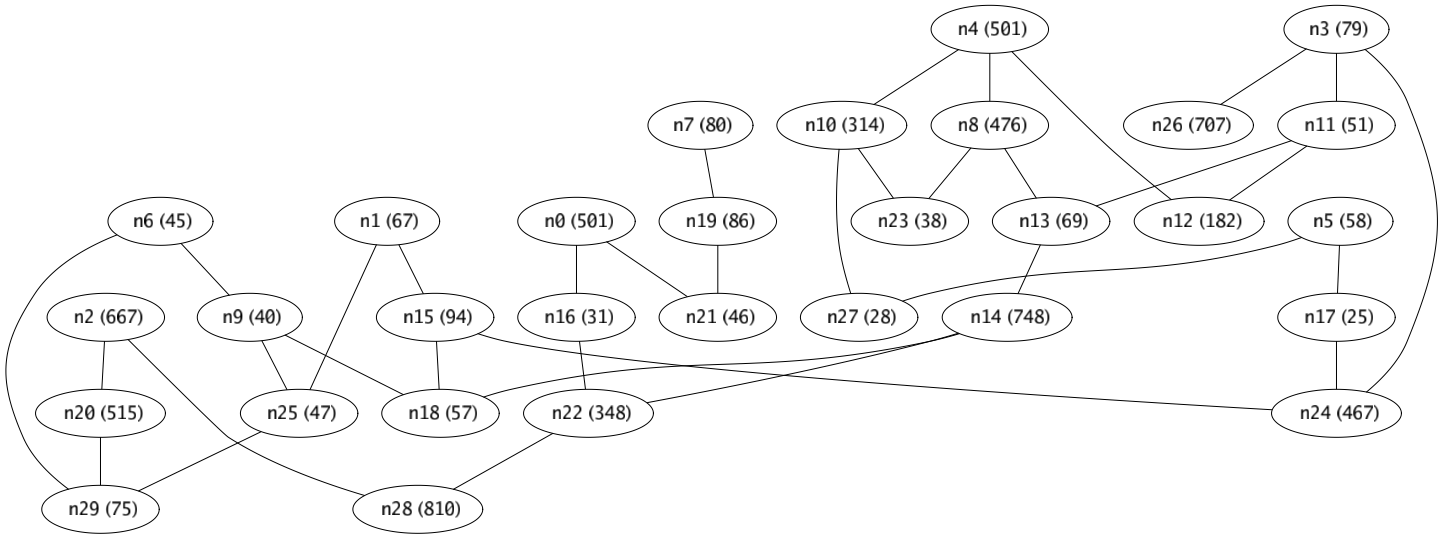
\includegraphics[scale=0.15]{img/graph-random.png}
\end{minipage}%
\begin{minipage}{.5\linewidth}
\centering
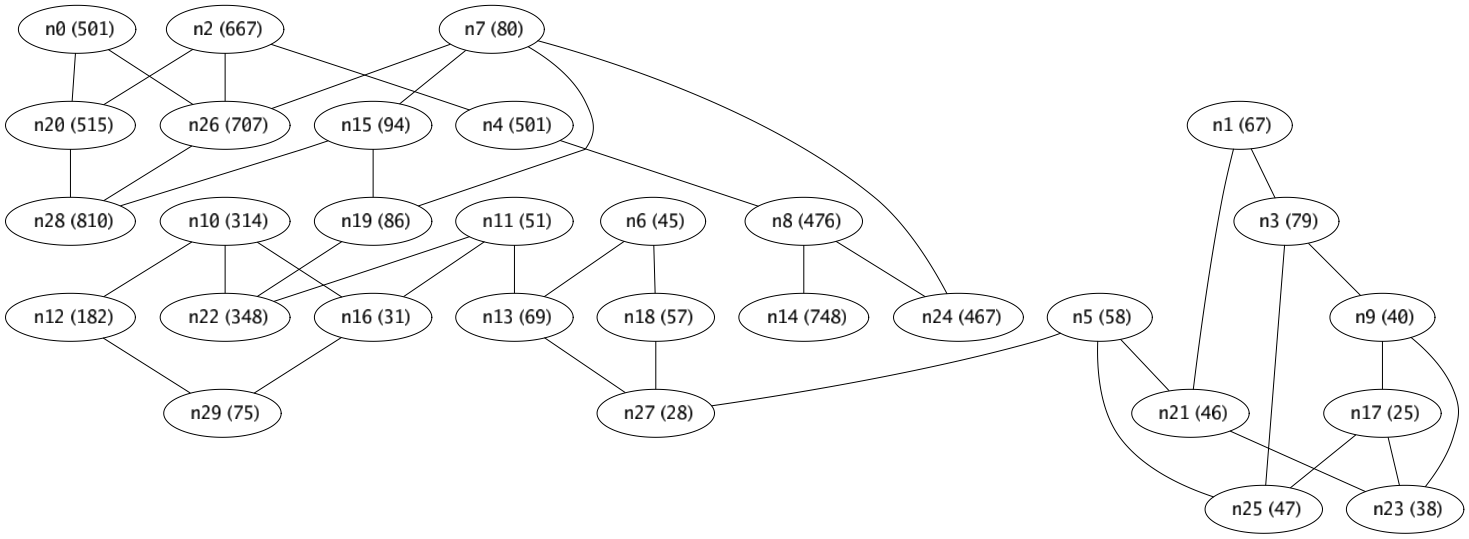
\includegraphics[scale=0.15]{img/graph-fat.png}
\end{minipage}
\caption{Two randomly generated overlays with average delays marked in parentheses. On the right a randomly wired one. On he left a fat-tree overlay.}
\end{figure}

Now we can see how the convergence behaves between these two graphs when simulated for 100 iterations. In the simulation we do not employ the "Most stragglers left behind" strategy.
Therefore it is expected for the total time of {\tt All} nodes of our simulation to be very close in both overlays. In the case of the fat tree structure for 20 experiments
the average time of convergence was 1m 38,2 seconds seconds while  for the random overlay the same average was 1m 40,5 seconds which for 100 iterations run
gives us minor speedup of approximately 2\%. The convergence behavior though is drastically different. In the following diagrams we can see in each
at 10s snapshots, the remaining iterations for fastest converging node, for the slowest converging node, and also the average iterations that were completed for that 10s interval.
\begin{figure}
\centering
\begin{minipage}{.5\linewidth}
\centering
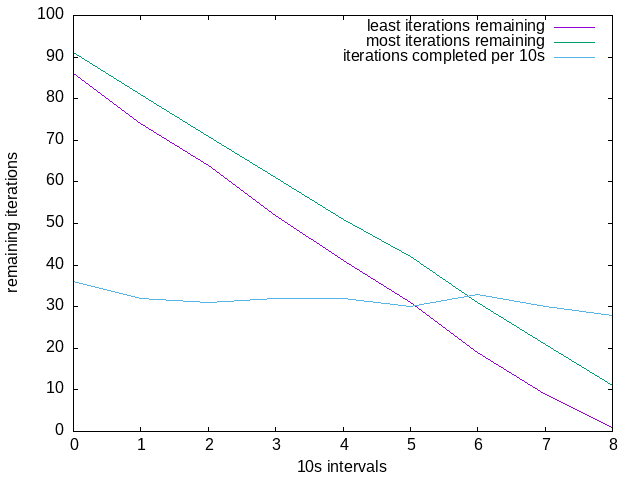
\includegraphics[scale=0.4]{img/random-1m40.png}
\end{minipage}%
\begin{minipage}{.5\linewidth}
\centering
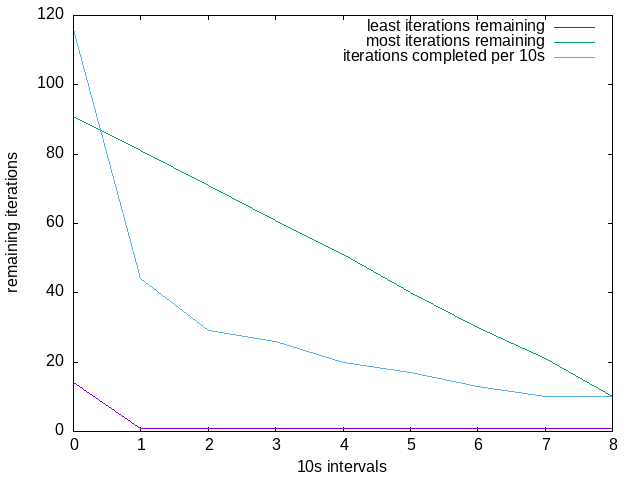
\includegraphics[scale=0.4]{img/fat-1m38.png}
\end{minipage}
\caption{On the left the convergence profile of the random overlay versus the one of the fat tree on the right}
\end{figure}
From the above diagram we believe that if we accept a computation loss of a v small part of the network, the speedup we will gain will be logarithmic
to the number of remaining nodes. As we also saw above , by expecting a small amount of the computation to fail too, we gain fault tolerant properties
for the remaining participants.
We intend to perform more runs and also investigate how the same properties scale according to the number of nodes and the number of iterations. Once a good
overlay topology based on local delay is established we will begin the implementation of the DHT variant of it in the sense of implementing the key function
that would shape it accordingly.

\section{Closing Remarks and Future Work}
As we see the choice of delay as parameter for the formation of neighborhoods on an overlay graph seems promising. It allows significantly larger 
throughputs in the initial runs of an algorithm and slight overall wall time improvement. If we are interested in having most of our nodes converge
faster then it makes a great choice for an overlay graph. We also see how the delay, being a local property, combined with a DHT can allow a node
to detect neighbours based either on that property, either on network proximity, or both, and we have sketched a way to move forward with an implementation.
We still need to implement the DHT for which we have began work that would require approximately 2 months for completion. Apart from the DHT the straggler strategy
needs to implemented in the simulator as well as the reliable message delivery mechanism.

\bibliographystyle{plain}
\bibliography{filo.bib}
\end{document}
